\chapter[Proposal]{Proposal}
\label{chap:proposal}

This proposal focuses on detailing the necessary steps to the creation and publication of a crowdfunding speech corpus in Brazilian Portuguese. To this end, a virtual voice recording application will be developed (section \ref{sec:proposal-app}), focusing on adding gamification elements to enhance user engagement. Additionally, this application will also extract some relevant characteristics found in the systematic literature review in chapter \ref{chap:slr}, such as speaker demographics. Once the construction is finished, the application will be released, allowing general public submission (in section \ref{sec:proposal-public-submission}). After the submission period, the collected data will be analyzed and compiled to a speech corpus (\ref{sec:proposal-data-analysis}), which will be publicized to an open-source repository in section \ref{sec:proposal-data-publication}.

\section{Application}
\label{sec:proposal-app}

This section details the conception, documentation, and development process of the voice recording application, coined "Fale Alguma Coisa". Below, it will at times be referenced as "app", short for application. The main purpose of this app is to be able to record predetermined phrases from users. All other features support the engagement and usability through authentication, gamification, and explanatory elements. 

Hence, the concept will be detailed, followed by the target audience (\ref{sec:app-concept} and \ref{sec:app-audience}). Secondly, the functionality of the entire application will be documented using user stories (\ref{sec:app-stories}), based on the concept and target audience. Thirdly, the design will be elaborated by documenting the layouts (in \ref{sec:app-design}) based on the user stories listed. One key factor in the app is the ability to teach science facts and trivia, which entails the need of proper phrase selection methods. These methods will be explained in \ref{sec:app-phrase-selection}. Lastly, the development process will be described, with additional details on the tools selected (\ref{sec:app-development}).

\begin{figure}[ht]
    \centering
    \caption{Fale Alguma Coisa app Logo}
     
\includegraphics[width=\linewidth/2]{images/app/logo.jpg}
    \caption*{Source: Author}
    \label{fig:falealgumacoisa-logo}
\end{figure}

\subsection{Concept}
\label{sec:app-concept}

The Fale Alguma Coisa app should provide an easy gateway for you to contribute your voice while having fun and learning various science facts and curiosities.

\subsection{Target Audience}
\label{sec:app-audience}

Directed towards anyone interested in learning and contributing to science.

\subsection{User Stories}
\label{sec:app-stories}

The development of most software starts with its documentation. This work chose a user story approach to project documentation and lists them below, categorized by epic.

\subsubsection{Usability}

The usability epic details user stories related to the user experience with the app.

\begin{itemize}
    \item I, as a citizen, would like to contribute my voice using my mobile devices and desktop computer.
\end{itemize}


\clearpage
\subsection{Design}
\label{sec:app-design}

To ensure the development of the application is effective, an iterative design approach was taken. First, ideas for the app shaped a conceptual user journey. Second, this journey allowed the creation of layouts, which then passed through a validation process. Then, if aligned with the application concept, the layouts were developed. Otherwise, another design implementation occurred, undergoing further validation. The sections below detail the finalized artifacts.

\subsubsection{Color Scheme}

In color theory, colors are used to communicate meaning, but also affect mood, and perception \cite{agoston2013color}. The design color scheme defines a color palette to choose from when designing new visual elements. Applying the concept, a more colorful color scheme was chosen to lighten the mood of the application, as shown in figure \ref{fig:falealgumacoisa-color-scheme}.

\begin{figure}[ht]
    \centering
    \caption{Fale Alguma Coisa color scheme}
     
\includegraphics[width=.8\linewidth]{images/app/colors.png}
    \caption*{Source: Author}
    \label{fig:falealgumacoisa-color-scheme}
\end{figure}

\clearpage
\subsubsection{Splash Screen}

As the user first enter the application, a splash screen will be shown to welcome him (mobile version in figure \ref{fig:falealgumacoisa-splash-page-design}). It contains the logo and an animation to draw the user's attention. After the animation, the home will be shown.

\begin{figure}[ht]
    \centering
    \caption{Fale Alguma Coisa Splash Page design}
    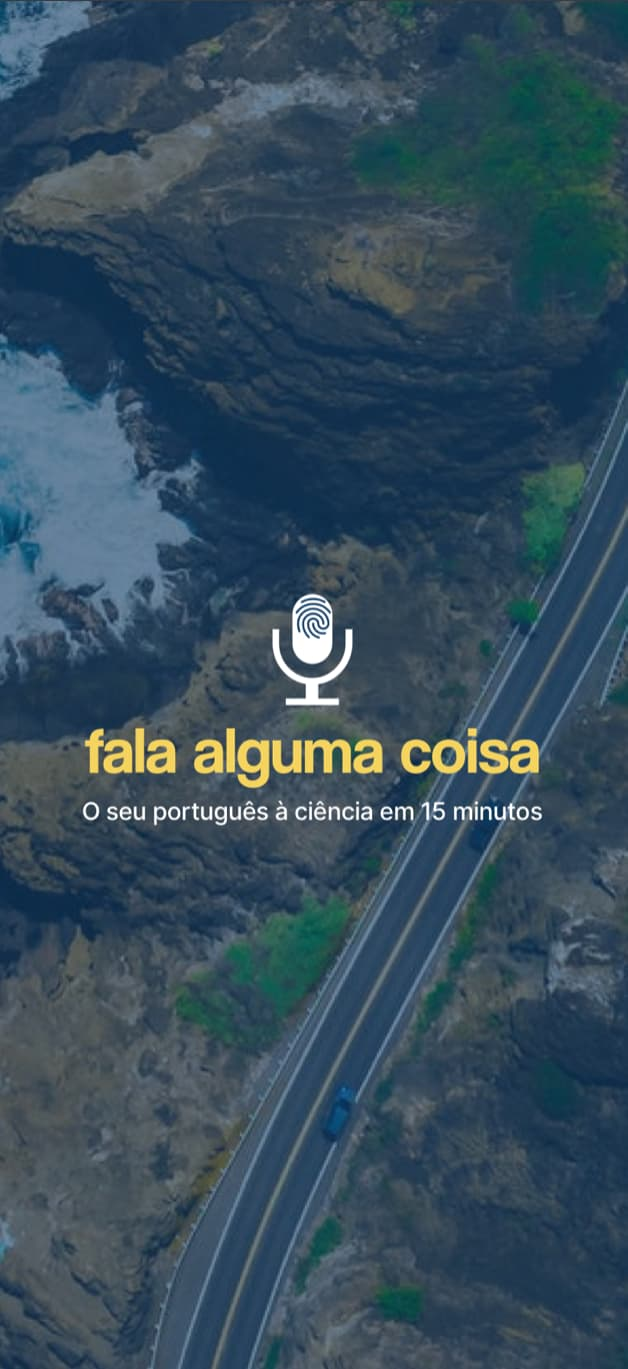
\includegraphics[width=\linewidth/2]{images/app/m-splash.jpg}
    \caption*{Source: Author}
    \label{fig:falealgumacoisa-splash-page-design}
\end{figure}

\subsubsection{Homepage}

After the splash animation, the homepage is shown. The mobile version can be seen below in figure \ref{fig:falealgumacoisa-home-page-design}. In this page, the call to action to start the recording is highlighted by the button at the center of the page, with text describing the project right below it. The login page is accessible through the link in the right upper corner. These few elements are placed to encourage the user to click on the recording, if he is a new user.

\begin{figure}[ht]
    \centering
    \caption{Fale Alguma Coisa Home Page design}
    \frame{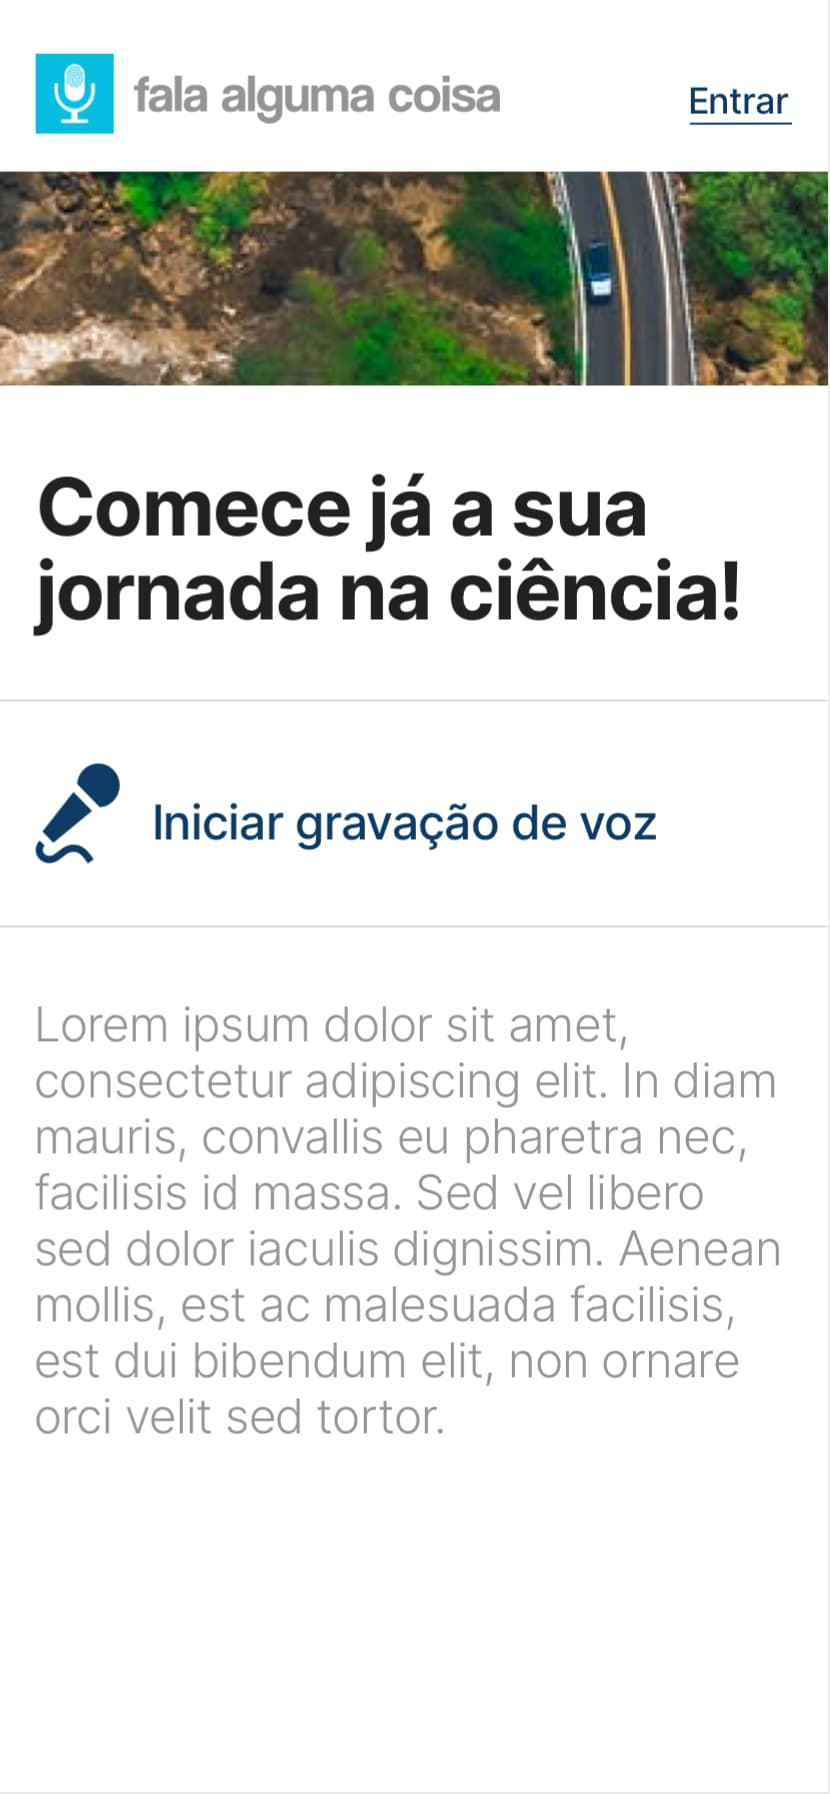
\includegraphics[width=\linewidth/2]{images/app/m-home.jpg}}
    \caption*{Source: Author}
    \label{fig:falealgumacoisa-home-page-design}
\end{figure}

\subsubsection{Recording}

This page represents the core functionality of the website, allowing the user to record phrases with his voice. The recording is done through groups of phrases, called a theme, and is illustrated by the image \ref{fig:falealgumacoisa-recording-page-design} at the bottom. The main elements of the page are (1) the phrase highlighted in a rectangular box at the center of the page, and (2) the red recording button at the bottom.

\begin{figure}[ht]
    \centering
    \caption{Fale Alguma Coisa Recording Page designs}
    \begin{subfigure}{.5\textwidth}
      \centering
      \frame{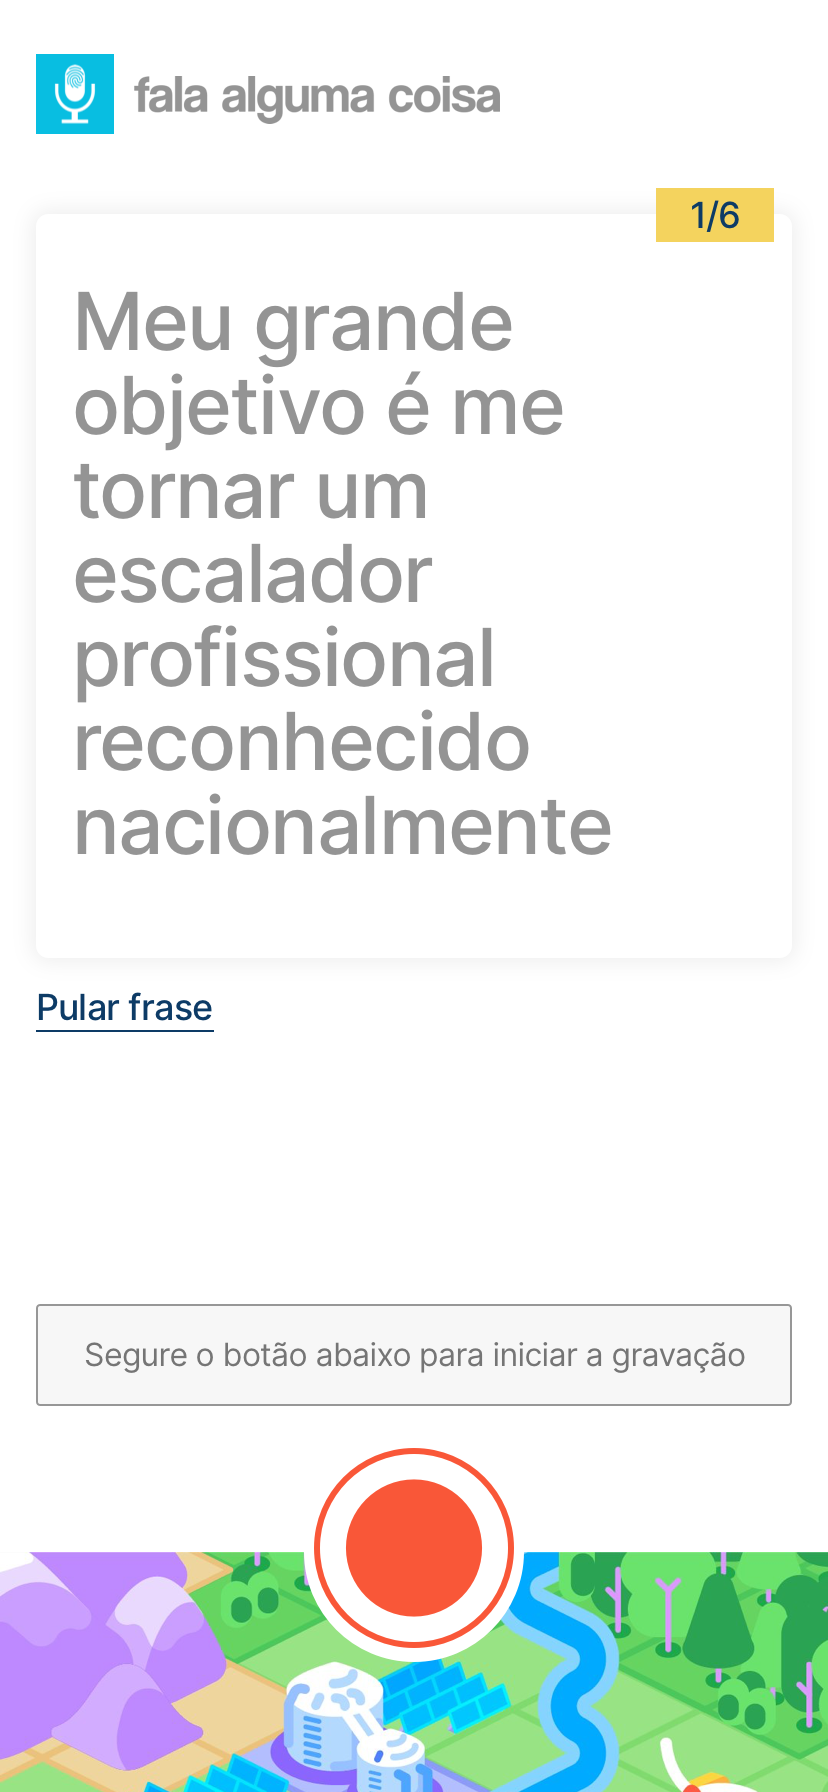
\includegraphics[width=.9\linewidth]{images/app/recording/Journey_1.0.png}}
      \caption{Waiting to start recording}
      \label{fig:falealgumacoisa-recording-page-design-start}
    \end{subfigure}%
    \begin{subfigure}{.5\textwidth}
      \centering
      \frame{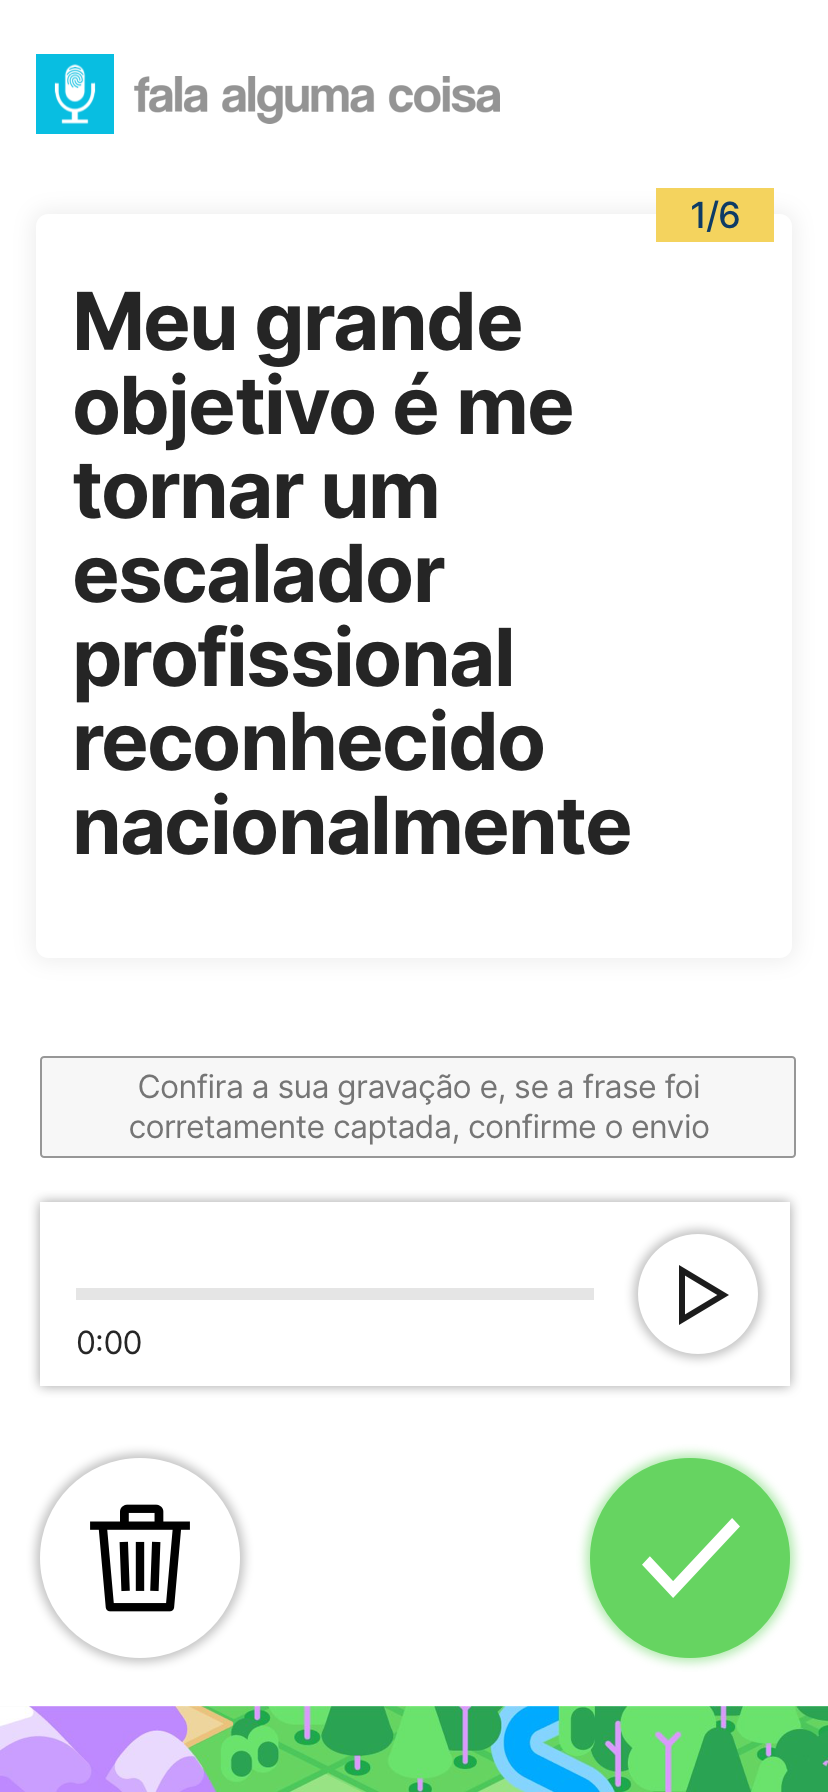
\includegraphics[width=.9\linewidth]{images/app/recording/Journey_1.2.png}}
      \caption{Confirm or delete recording}
      \label{fig:falealgumacoisa-recording-page-design-confirm}
    \end{subfigure}
    \caption*{Source: Author}
    \label{fig:falealgumacoisa-recording-page-design}
\end{figure}

\subsubsection{Terms of Service}

To comply with Brazil's General Data Protection Act (Law 13,709/2018), the application has to clarify data usage of the visitor of the website. The figure \ref{fig:falealgumacoisa-tos-page-design} defines the layout of the page with a simplified terms of service, as well as a button to accept or deny such terms.

\begin{figure}[ht]
    \centering
    \caption{Fale Alguma Coisa simplified terms of service page design}
    \frame{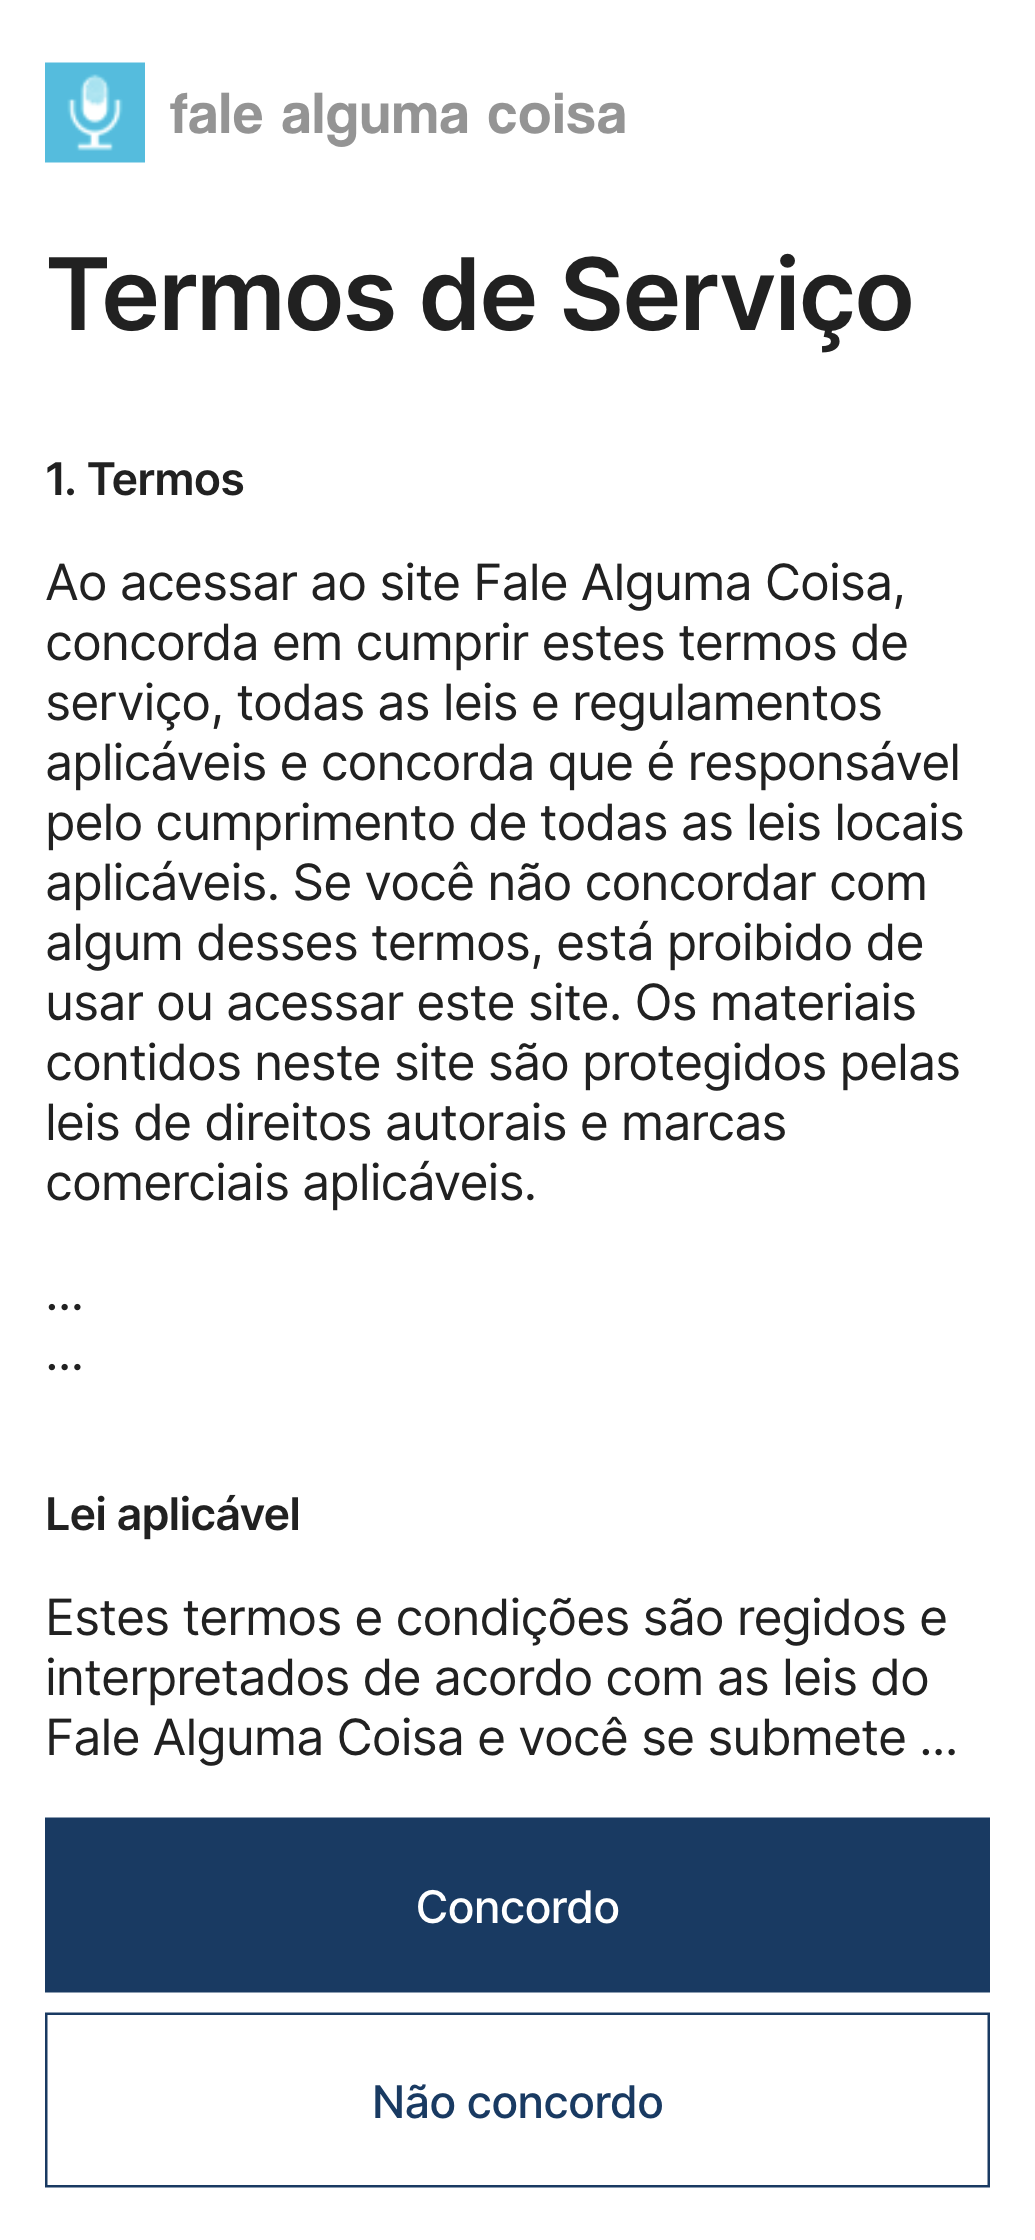
\includegraphics[width=\linewidth/2]{images/app/register/tos.png}}
    \caption*{Source: Author}
    \label{fig:falealgumacoisa-tos-page-design}
\end{figure}

\subsubsection{Dashboard}

When an unauthenticated user finishes recording its first theme, or when a user logs in, they are able to select from a list of themes to record. In this dashboard seen in figure \ref{fig:falealgumacoisa-dashboard-page-design}, they are also shown the number of points accumulated by the usage of the app, as well as able to open a menu and notification page.

\begin{figure}[ht]
    \centering
    \caption{Fale Alguma Coisa Dashboard Page design}
    \frame{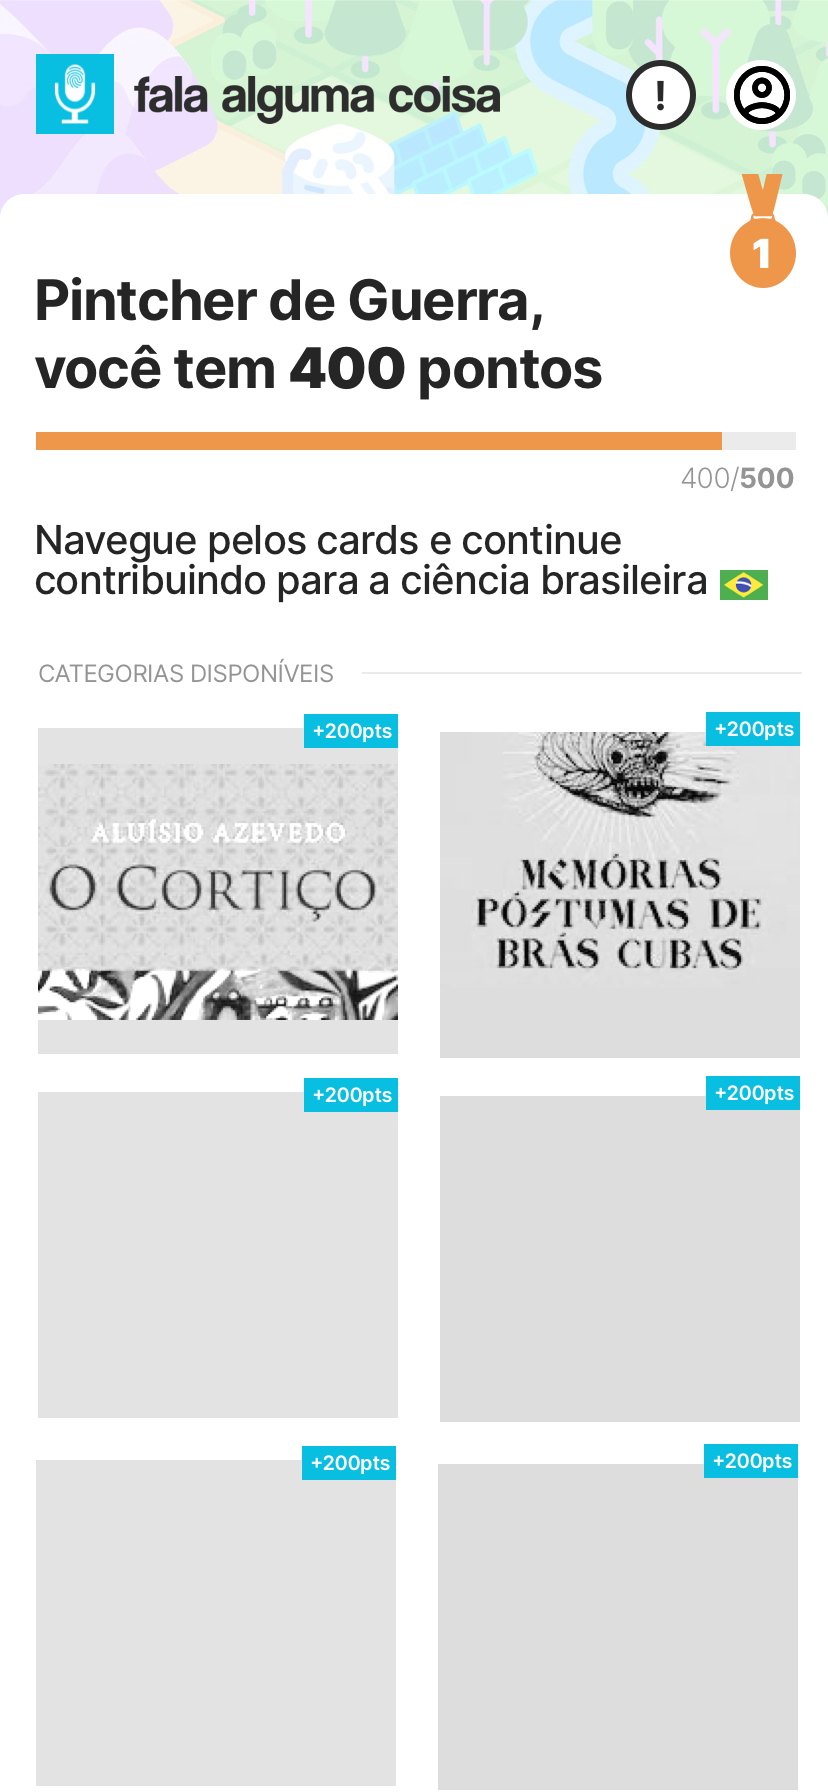
\includegraphics[width=\linewidth/2]{images/app/dashboard/Dashboard.png}}
    \caption*{Source: Author}
    \label{fig:falealgumacoisa-dashboard-page-design}
\end{figure}

\subsubsection{Leaderboard}

The leaderboard layouts feature two visualizations, depending on the desired scope. Should the contributor want to see all top ranking users, the leaderboard (figure \ref{fig:falealgumacoisa-leaderboard-page-design-general}) is available. If the user only wants to check his friend rankings, the application displays a reduced list (figure \ref{fig:falealgumacoisa-leaderboard-page-design-friend}), based on the friends added to the platform. These layouts provide a way for users to compare their contributions, thus promoting competition. A social element is also included throughout the option to add friends.

\begin{figure}[ht]
    \centering
    \caption{Fale Alguma Coisa Leaderboard Page designs}
    \begin{subfigure}{.5\textwidth}
      \centering
      \frame{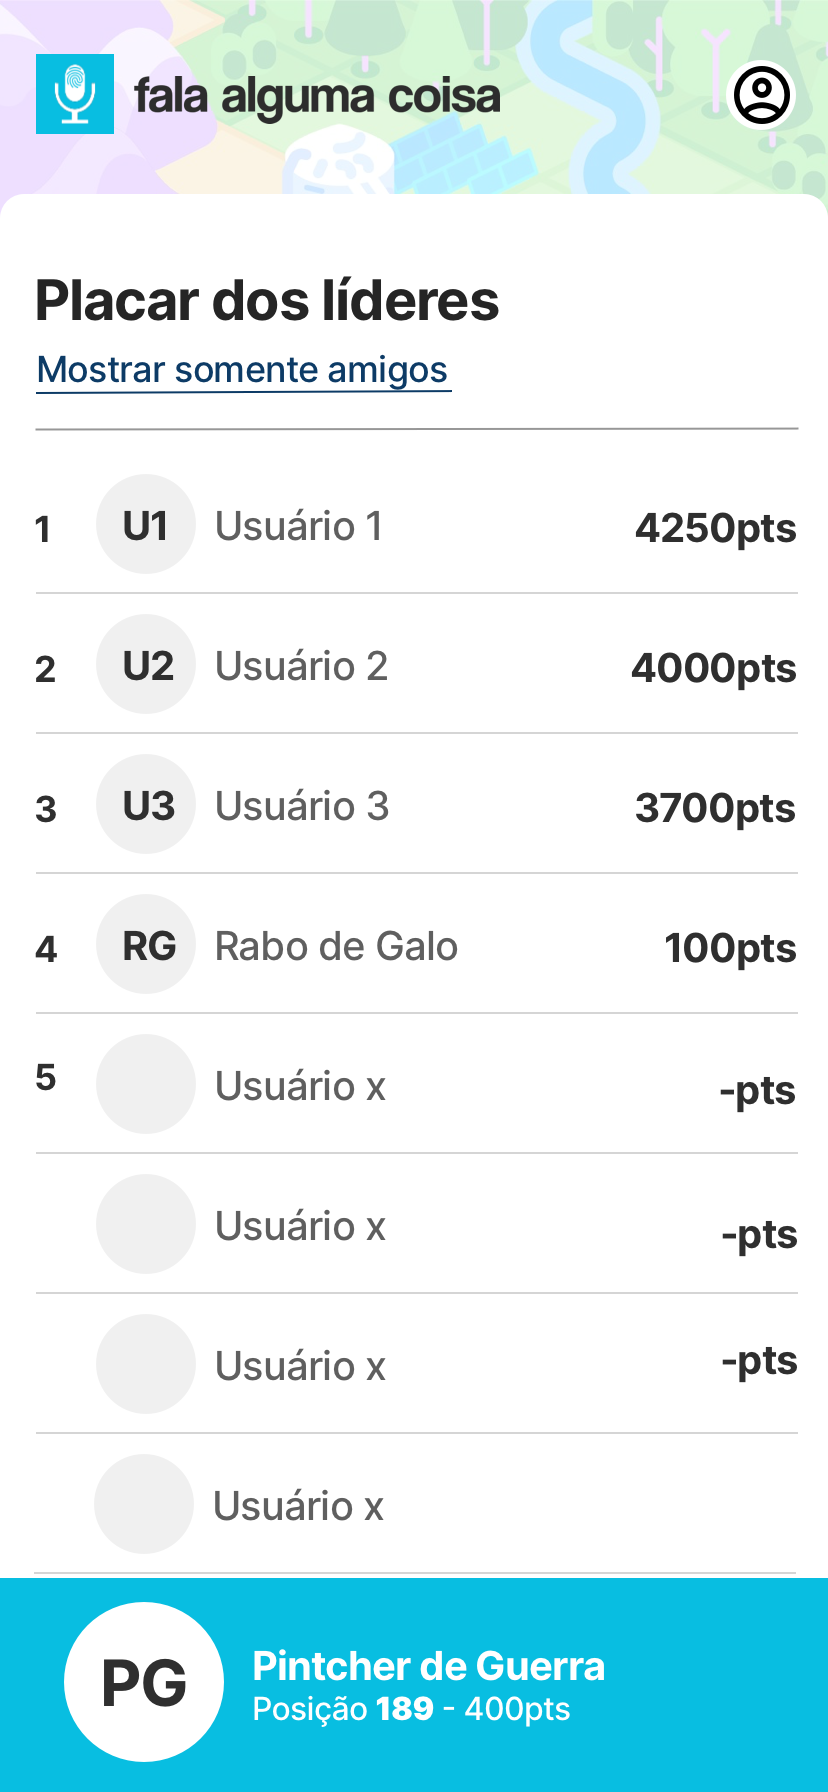
\includegraphics[width=.9\linewidth]{images/app/leaderboard/GeneralRanking.png}}
      \caption{General Leaderboard}
      \label{fig:falealgumacoisa-leaderboard-page-design-general}
    \end{subfigure}%
    \begin{subfigure}{.5\textwidth}
      \centering
      \frame{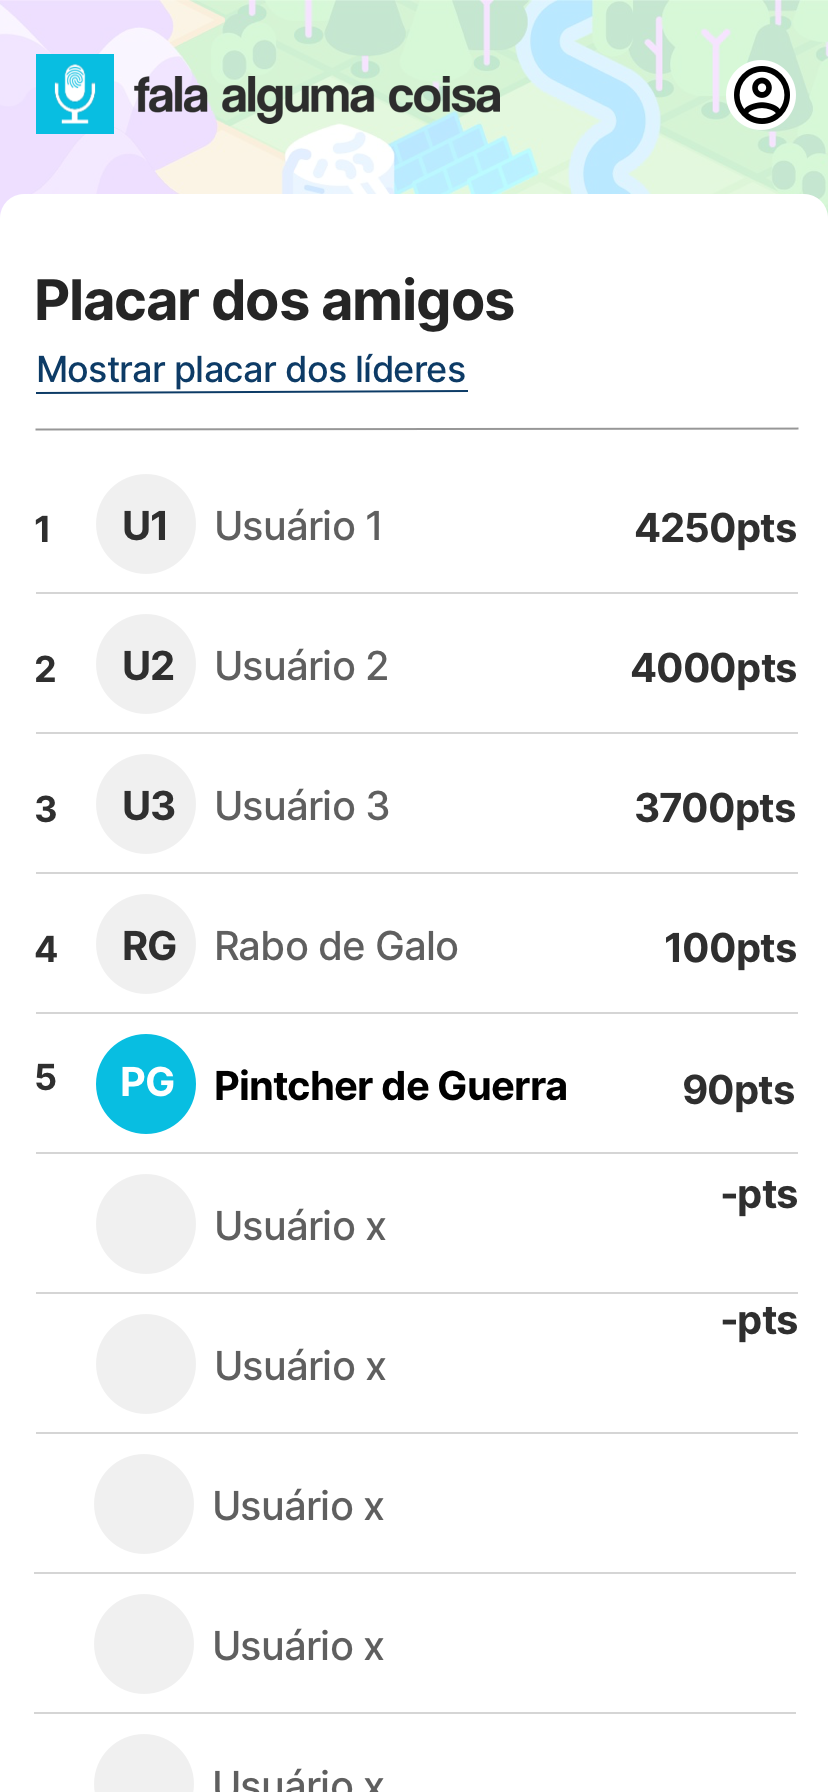
\includegraphics[width=.9\linewidth]{images/app/leaderboard/FriendsRanking.png}}
      \caption{Friends Leaderboard}
      \label{fig:falealgumacoisa-leaderboard-page-design-friend}
    \end{subfigure}
    \caption*{Source: Author}
    \label{fig:falealgumacoisa-leaderboard-page-design}
\end{figure}

\subsubsection{Friends}

The ability to add and track (follow) friends is possible with the layouts described below. If he knows the name of the user, the contributor can search for his friends using the Search Friends page (seen in figure \ref{fig:falealgumacoisa-friends-page-design-search}). The results return in the same page below the search input field (figure \ref{fig:falealgumacoisa-friends-page-design-results}), as a list of users. To add a friend, it is as simple as clicking the "Seguir" button in the right corner of the result list. This click toggles the button with a "Seguindo" text. If this new state is clicked, the friend is removed.

\begin{figure}[ht]
    \centering
    \caption{Fale Alguma Coisa Friends Page designs}
    \begin{subfigure}{.5\textwidth}
      \centering
      \frame{
\includegraphics[width=.9\linewidth]{images/app/friends/FriendsSearch_1.0.png}}
      \caption{Search for friends}
      \label{fig:falealgumacoisa-friends-page-design-search}
    \end{subfigure}%
    \begin{subfigure}{.5\textwidth}
      \centering
      \frame{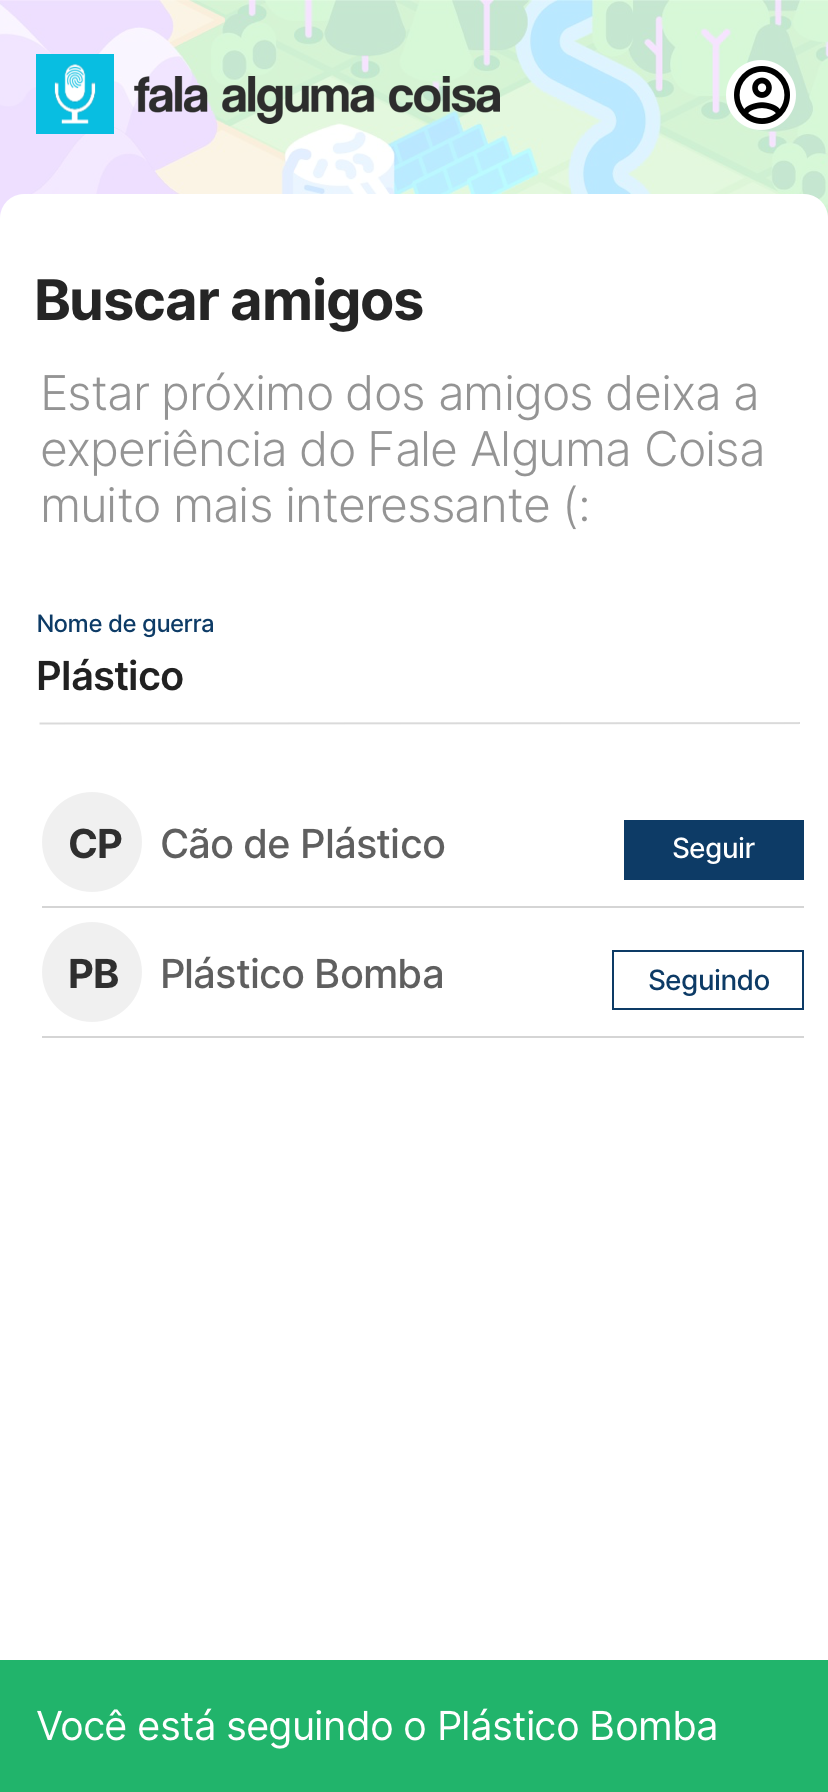
\includegraphics[width=.9\linewidth]{images/app/friends/FriendsSearch_1.3.png}}
      \caption{Search friends results}
      \label{fig:falealgumacoisa-friends-page-design-results}
    \end{subfigure}
    \caption*{Source: Author}
    \label{fig:falealgumacoisa-friends-page-design}
\end{figure}

\subsubsection{Refer Friends}

To earn more contribution points, the citizen scientist can also refer new friends using the Refer friends page. The mobile version of this page is illustrated in figure \ref{fig:falealgumacoisa-refer-page-design}, and has one button "Compartilhar", which enables the mobile sharing functionality. The link shared redirects to a registration page, and both users get 100 points after the registration of the reffered user.

\begin{figure}[ht]
    \centering
    \caption{Fale Alguma Coisa Refer Friends Page design}
    \frame{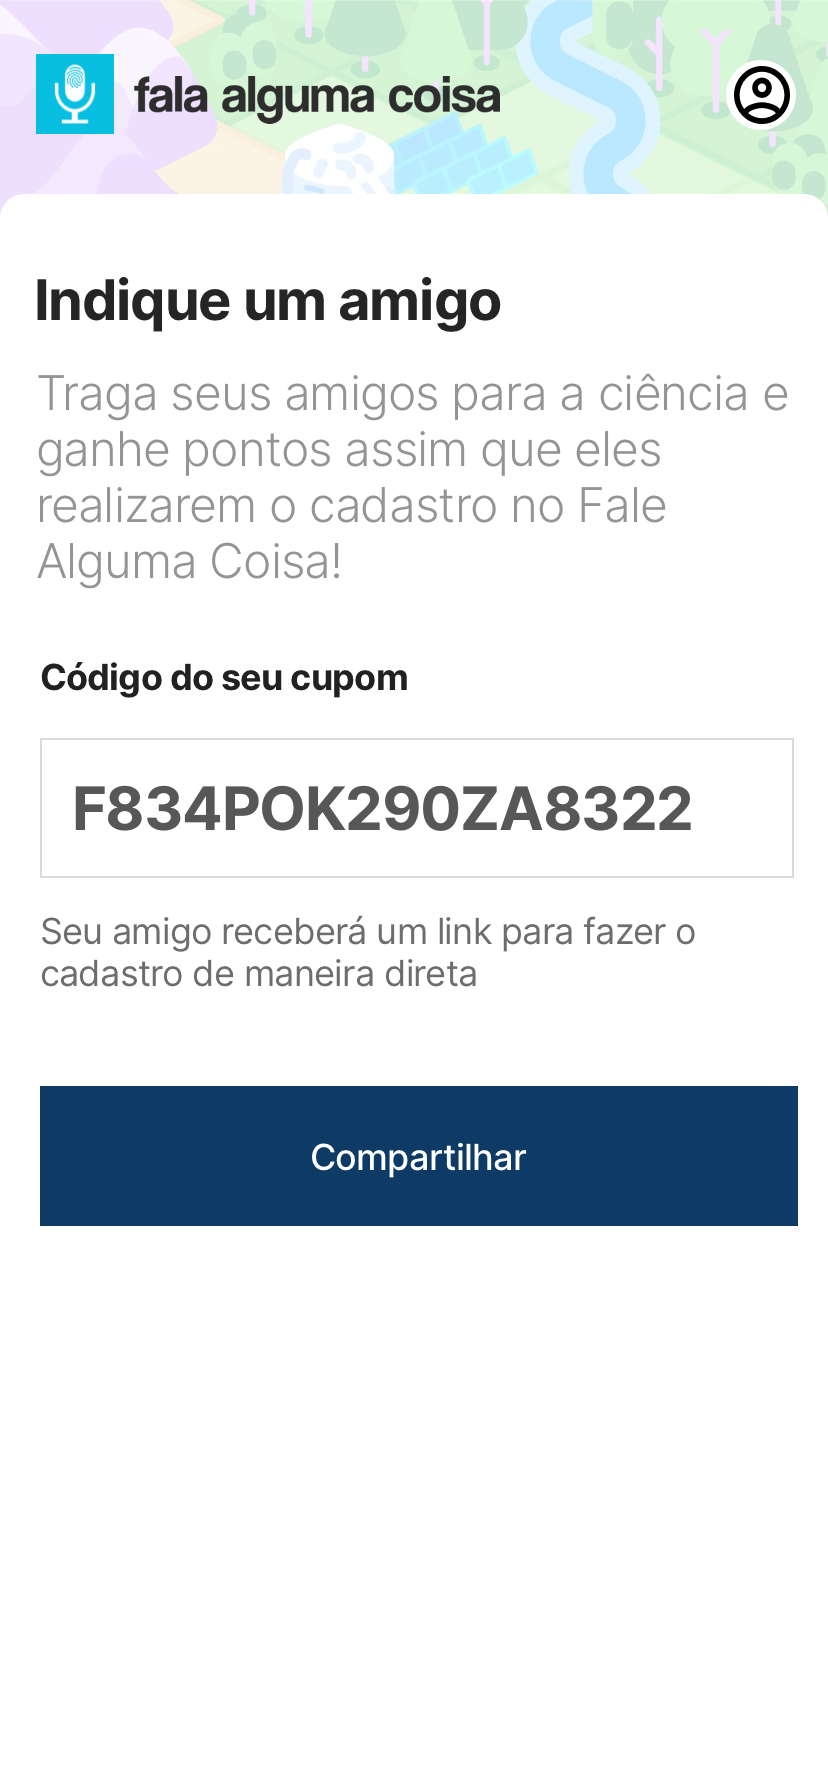
\includegraphics[width=\linewidth/2]{images/app/friends/Search_Friend_1.0.png}}
    \caption*{Source: Author}
    \label{fig:falealgumacoisa-refer-page-design}
\end{figure}

\subsubsection{Login and Registration}

The login and registration pages include essential features to the application: the ability to identify the user and maintain a history of recordings. The figure in \ref{fig:falealgumacoisa-login-page-design} represents a login flow possible to the contributor - using a username and password. It is also possible to use the "social login" through Facebook and Google, identifiable by the respective buttons in the layout.

\begin{figure}[ht]
    \centering
    \caption{Fale Alguma Coisa Login Page designs}
    \begin{subfigure}{.5\textwidth}
      \centering
      \frame{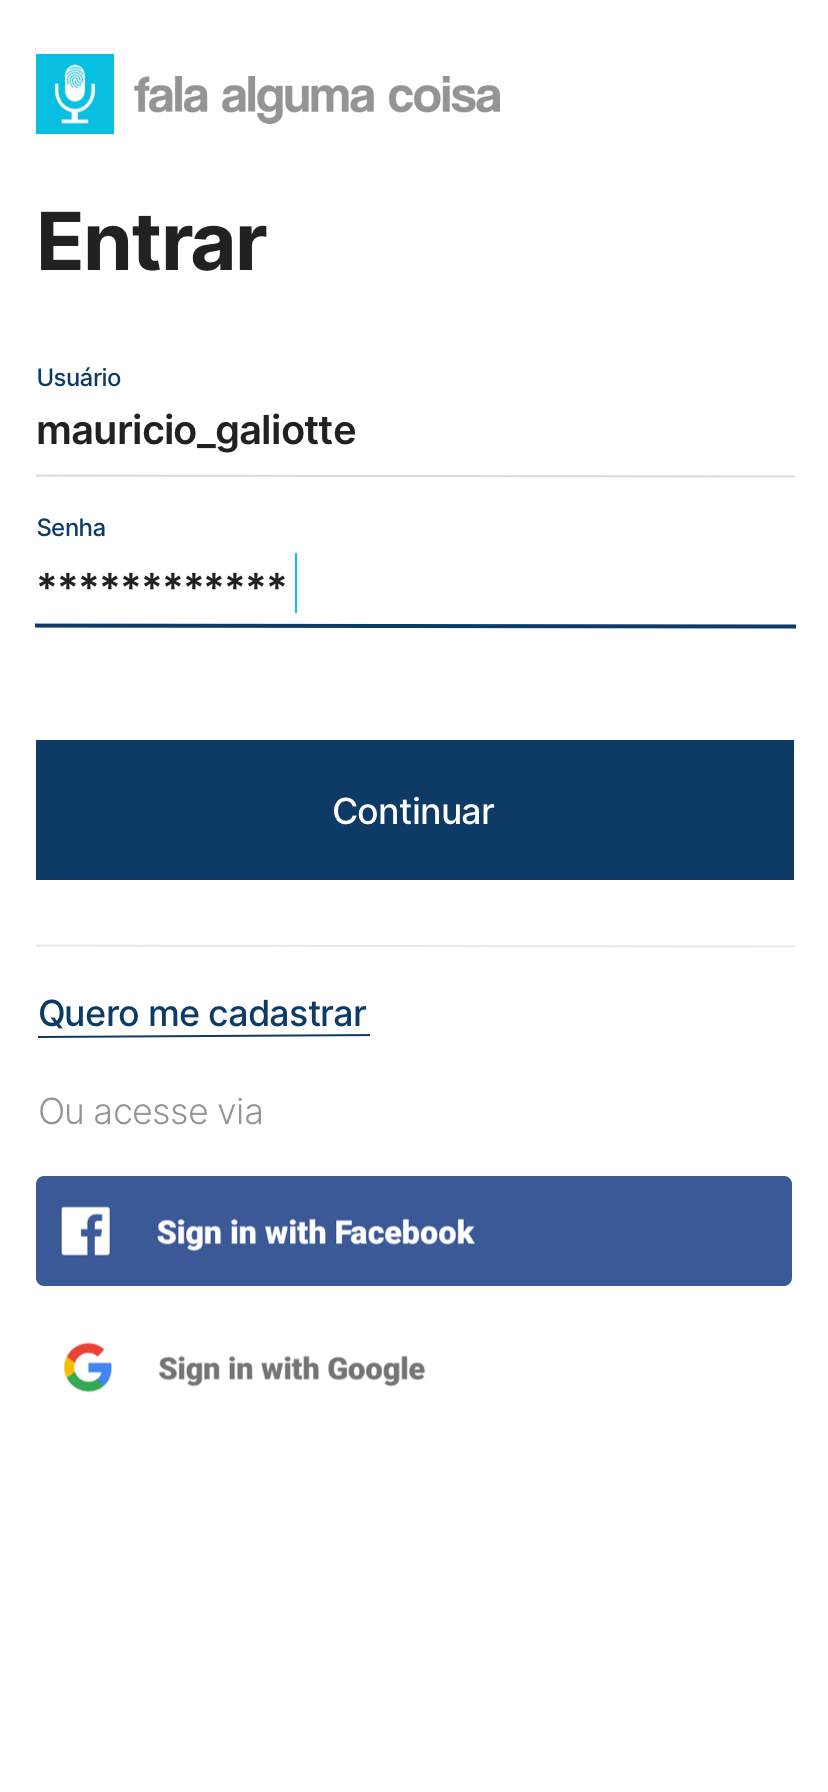
\includegraphics[width=.9\linewidth]{images/app/login/Login2.png}}
      \caption{Login with email and password}
      \label{fig:falealgumacoisa-login-page-design}
    \end{subfigure}%
    \begin{subfigure}{.5\textwidth}
      \centering
      \frame{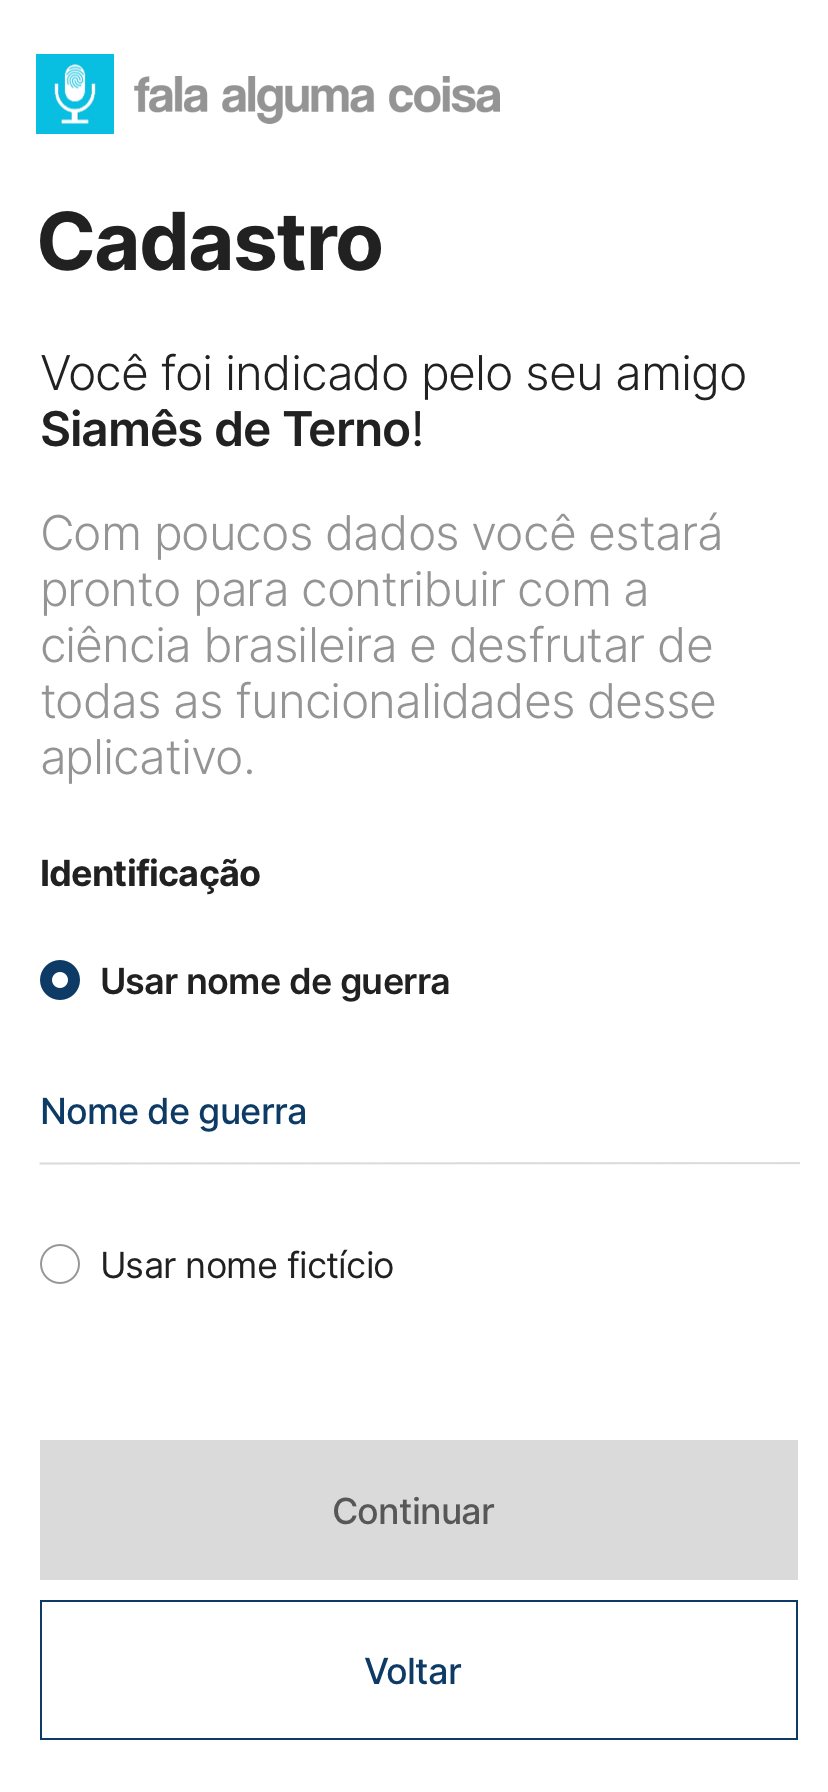
\includegraphics[width=.9\linewidth]{images/app/register/Register1.0.png}}
      \caption{Registration with \textit{pen name} selection}
      \label{fig:falealgumacoisa-registration-page-design-pen-name}
    \end{subfigure}
    \caption*{Source: Author}
    \label{fig:falealgumacoisa-login-and-registration-page-design}
\end{figure}

To register with the Fale Alguma Coisa app, the user must choose his \textit{pen name} (figure \ref{fig:falealgumacoisa-registration-page-design-pen-name}) and add some demographics information (seen in figure \ref{fig:falealgumacoisa-registration-page-design-demographics}. The registration flow can be triggered in two ways, and each have their differences:

\begin{itemize}
    \item Using the "social login" button. In this format, the user authenticates using the social media account and therefore does not need to provide email and password. Subsequent logins should use this method as well.
    \item Using a manual registration button ("Quero me cadastrar"). In addition to the name and demographics, the user must also provide his email and password as a last step (figure \ref{fig:falealgumacoisa-registration-page-design-email-password}).
\end{itemize}

\begin{figure}[ht]
    \centering
    \caption{Fale Alguma Coisa Registration steps designs}
    \begin{subfigure}{.5\textwidth}
      \centering
      \frame{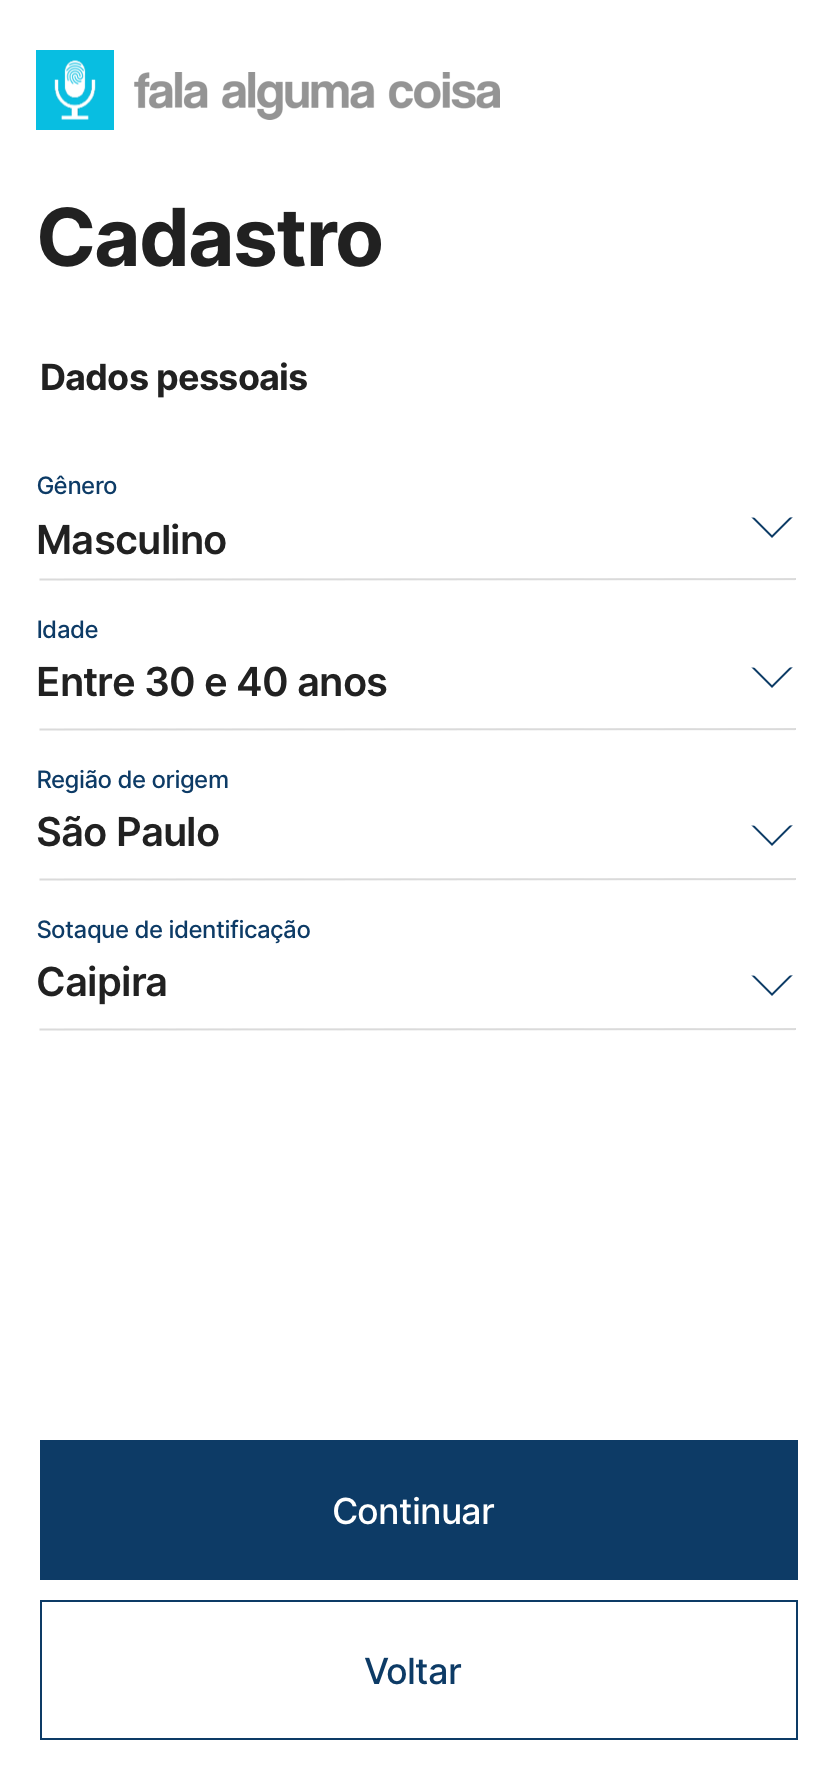
\includegraphics[width=.9\linewidth]{images/app/register/Register2.1.png}}
      \caption{Demographics step}
      \label{fig:falealgumacoisa-registration-page-design-demographics}
    \end{subfigure}%
    \begin{subfigure}{.5\textwidth}
      \centering
      \frame{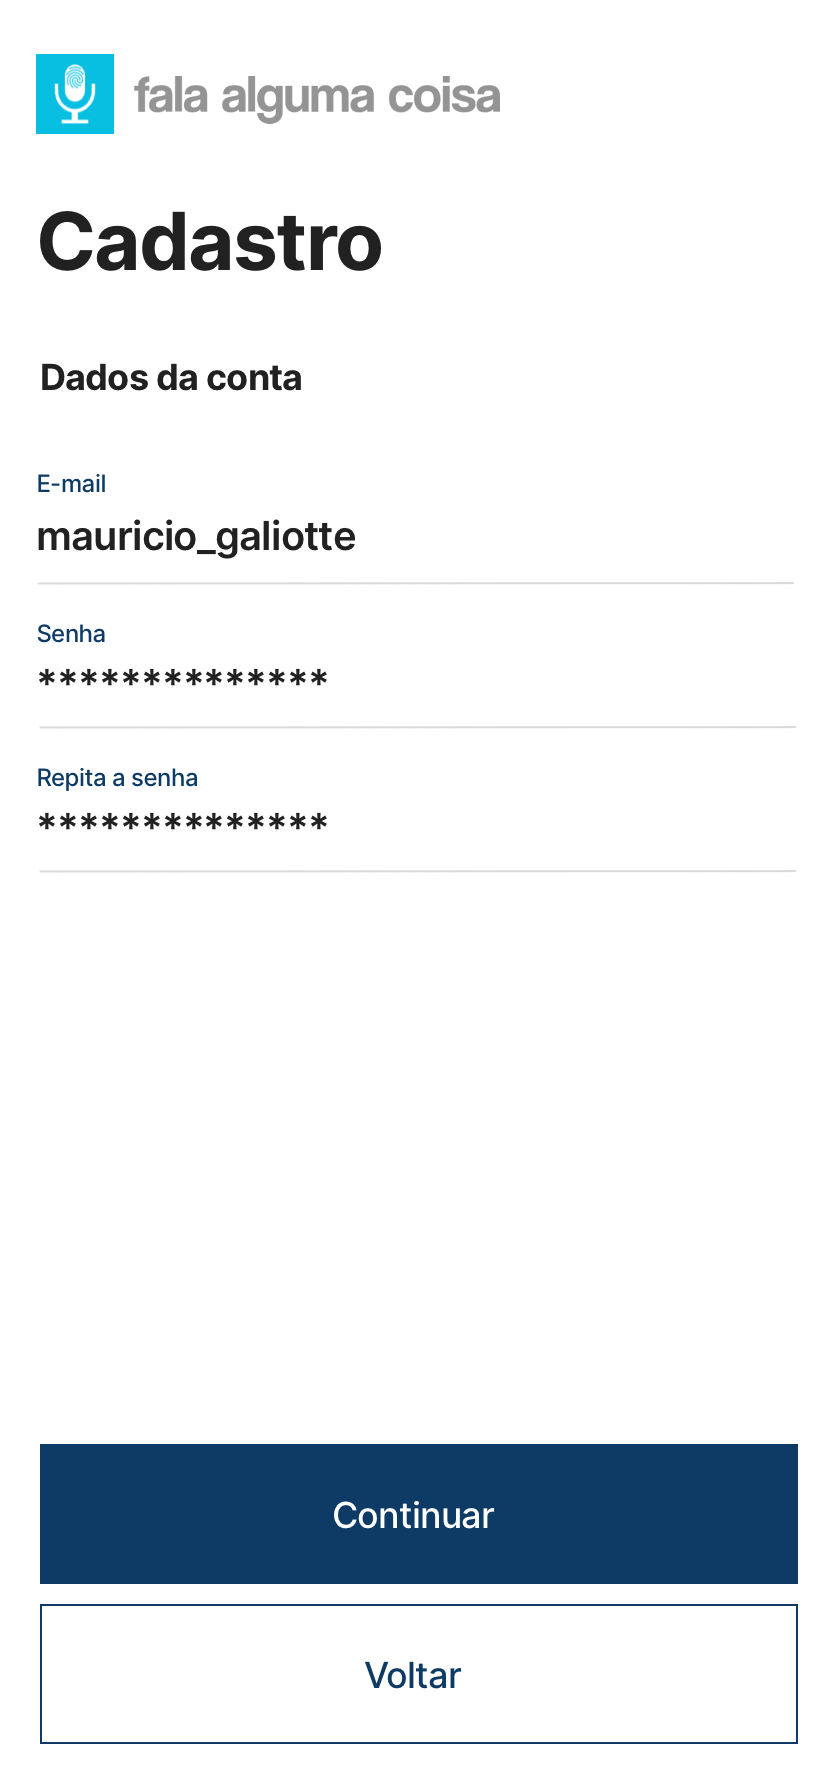
\includegraphics[width=.9\linewidth]{images/app/register/Register3.0.png}}
      \caption{Email and password step}
      \label{fig:falealgumacoisa-registration-page-design-email-password}
    \end{subfigure}
    \caption*{Source: Author}
    \label{fig:falealgumacoisa-registration-page-design}
\end{figure}

\subsubsection{Delete User}

If necessary, the user should be able to delete its user data, while still contributing his voice to the speech corpus. The following figures (\ref{fig:falealgumacoisa-delete-user-data-page-design-1} and \ref{fig:falealgumacoisa-delete-user-data-page-design-2}) include the design of the layout for this deletion flow.

\begin{figure}[ht]
    \centering
    \caption{Fale Alguma Coisa Delete User Data steps designs}
    \begin{subfigure}{.5\textwidth}
      \centering
      \frame{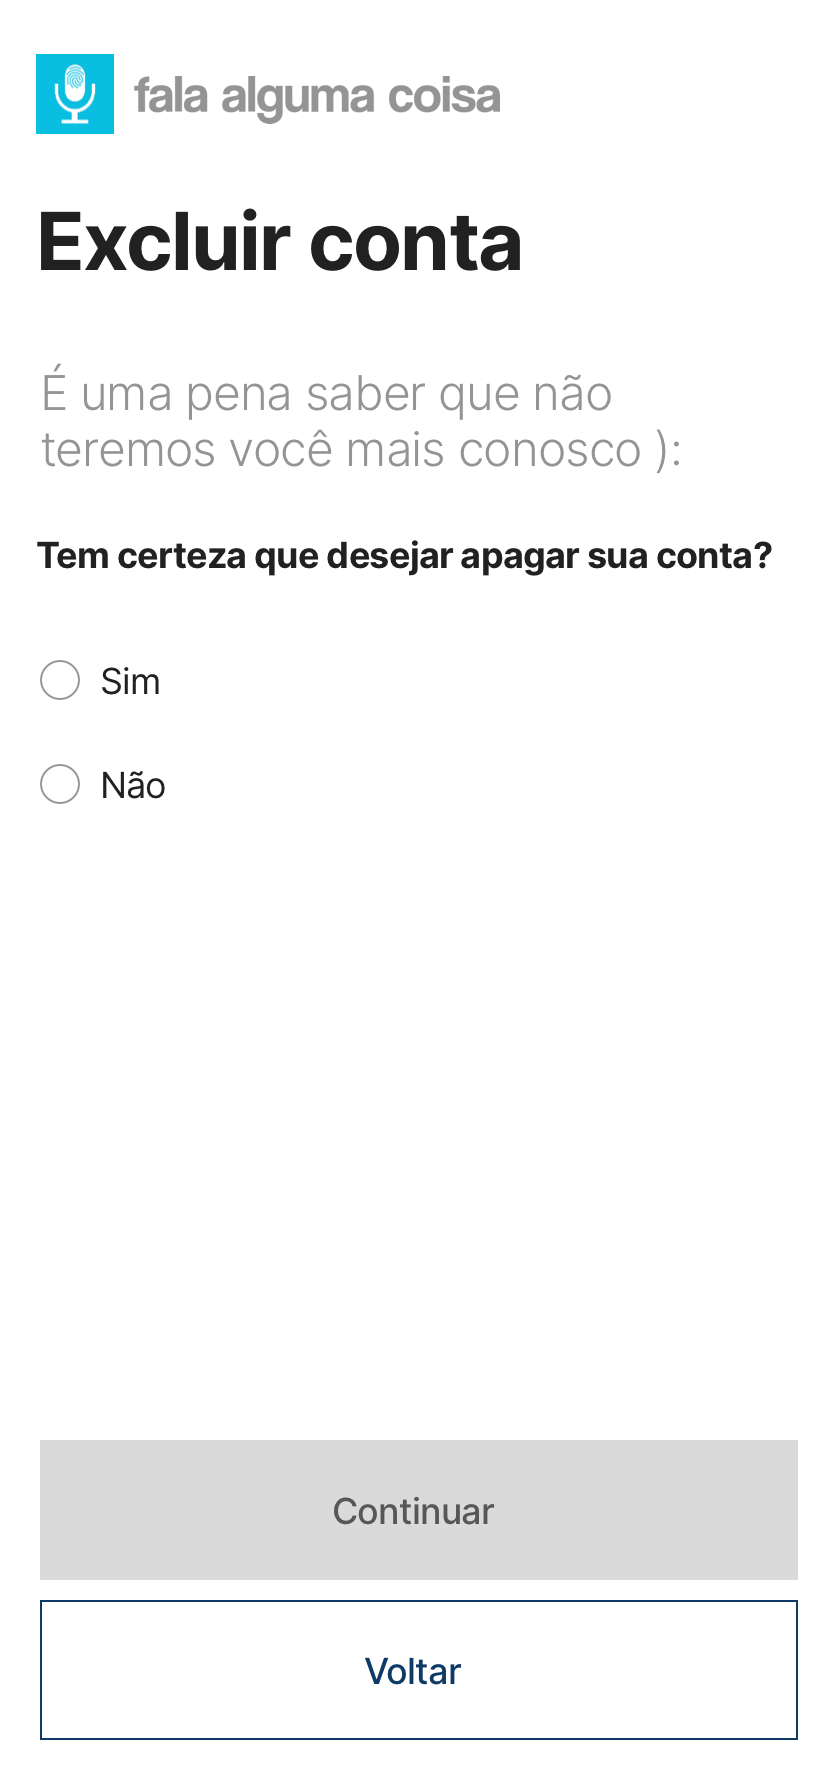
\includegraphics[width=.9\linewidth]{images/app/delete-user/FinishAccount1.0.png}}
      \caption{Deletion confirmation}
      \label{fig:falealgumacoisa-delete-user-data-page-design-1}
    \end{subfigure}%
    \begin{subfigure}{.5\textwidth}
      \centering
      \frame{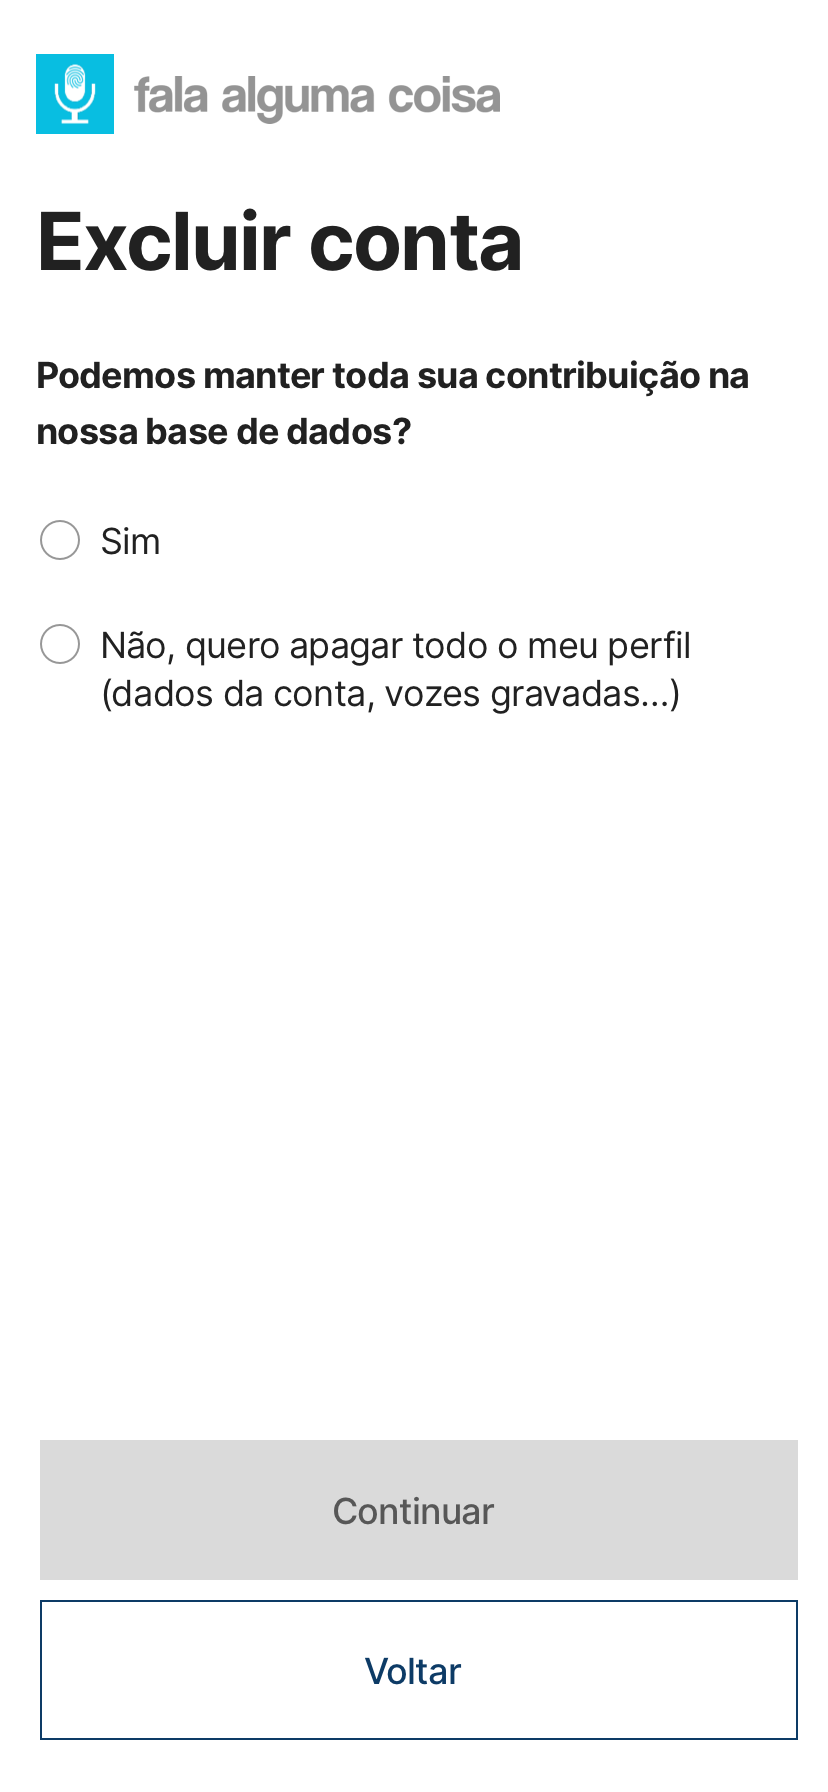
\includegraphics[width=.9\linewidth]{images/app/delete-user/FinishAccount2.0.png}}
      \caption{Scope of deletion}
      \label{fig:falealgumacoisa-delete-user-data-page-design-2}
    \end{subfigure}
    \caption*{Source: Author}
    \label{fig:falealgumacoisa-delete-user-data-page-design}
\end{figure}

\clearpage
\subsection{Phrase Selection}
\label{sec:app-phrase-selection}

\subsection{Development}
\label{sec:app-development}

This section details the development process of the Fale Alguma Coisa app.

\subsubsection{Web app}

To allow easier access to the voice recording app, a web-based application will be developed. This factor positively influences the capacity of the app to update over time, when compared to an application developed in a native environment. It also enables users over mobile and desktop to access the same application, and although the layout may have to be redesigned, most logic is reused.

\subsubsection{Mobile First}

The design will use a mobile first approach, to ensure the user flow will be optimized when he is using a mobile device. The desktop flow will be designed and developed afterwards.

\subsubsection{Tools Selection}

To develop the application, a selection of tools was made. The table \ref{tab:tools-selection} details the selected tools and explains each choice.

\begin{table}[h]
    \centering
    \begin{tabular}{|c|c|c|}
        \hline Category & Selection & Explanation \\
        \hline Design & Zeplin & Easy sharing  \\ 
        \hline Desig &  & access \\ 
        \hline Galaxy Zoo & access & access \\ 
        \hline Christmas Audubom Birdwatch & access & access \\ \hline 
    \end{tabular}
    \caption{Contribution for online citizen science projects}
    \label{tab:cs-contributions}
\end{table}


\section{General Public Submission}
\label{sec:proposal-public-submission}

\section{Data Analysis}
\label{sec:proposal-data-analysis}

\section{Data Publication}
\label{sec:proposal-data-publication}